\documentclass[draft=false
              ,paper=a4
              ,twoside=false
              ,fontsize=11pt
              ,headsepline
              ,BCOR10mm
              ,DIV11
              ]{scrbook}
\usepackage[ngerman,english]{babel}
%% see http://www.tex.ac.uk/cgi-bin/texfaq2html?label=uselmfonts
\usepackage[T1]{fontenc}
%\usepackage[utf8]{inputenc}
\usepackage[latin1]{inputenc}
\usepackage{libertine}
\usepackage{pifont}
\usepackage{microtype}
\usepackage{textcomp}
\usepackage[german,refpage]{nomencl}
\usepackage{setspace}
\usepackage{makeidx}
\usepackage{listings}
\usepackage{natbib}
\usepackage[ngerman,colorlinks=true]{hyperref}
\usepackage{soul}
\usepackage{hawstyle}
\usepackage{lipsum} %% for sample text

%% define some colors
\colorlet{BackgroundColor}{gray!20}
\colorlet{KeywordColor}{blue}
\colorlet{CommentColor}{black!60}
%% for tables
\colorlet{HeadColor}{gray!60}
\colorlet{Color1}{blue!10}
\colorlet{Color2}{white}

%% configure colors
\HAWifprinter{
  \colorlet{BackgroundColor}{gray!20}
  \colorlet{KeywordColor}{black}
  \colorlet{CommentColor}{gray}
  % for tables
  \colorlet{HeadColor}{gray!60}
  \colorlet{Color1}{gray!40}
  \colorlet{Color2}{white}
}{}
\lstset{%
  numbers=left,
  numberstyle=\tiny,
  stepnumber=1,
  numbersep=5pt,
  basicstyle=\ttfamily\small,
  keywordstyle=\color{KeywordColor}\bfseries,
  identifierstyle=\color{black},
  commentstyle=\color{CommentColor},
  backgroundcolor=\color{BackgroundColor},
  captionpos=b,
  fontadjust=true
}
\lstset{escapeinside={(*@}{@*)}, % used to enter latex code inside listings
        morekeywords={uint32_t, int32_t}
}
\ifpdfoutput{
  \hypersetup{bookmarksopen=false,bookmarksnumbered,linktocpage}
}{}

%% more fancy C++
\DeclareRobustCommand{\cxx}{C\raisebox{0.25ex}{{\scriptsize +\kern-0.25ex +}}}

\clubpenalty=10000
\widowpenalty=10000
\displaywidowpenalty=10000

% unknown hyphenations
\hyphenation{
}

%% recalculate text area
\typearea[current]{last}

\makeindex
\makenomenclature

\begin{document}
\selectlanguage{ngerman}

%%%%%
%% customize (see readme.pdf for supported values)
\HAWThesisProperties{Author={Ivan Morozov}
                    ,Title={Anomaly Detection in Financial Data by Using Machine Learning Methods}
                    ,EnglishTitle={Anomaly Detection in Financial Data by using Machine Learning Methods}
                    ,ThesisType={Masterarbeit}
                    ,ExaminationType={Masterprüfung}
                    ,DegreeProgramme={Master of Science Angewandte Informatik}
                    ,ThesisExperts={Prof. Dr. Kai von Luck \and Prof. Dr. Klaus-Peter Schoeneberg}
                    ,ReleaseDate={1. Januar 2345}
                  }

%% title
\frontmatter

%% output title page
\maketitle

\onehalfspacing

%% add abstract pages
%% note: this is one command on multiple lines
\HAWAbstractPage
%% German abstract
{Maschinelles Lernen, Betrugserkennung, Finanzdaten, Datenverarbeitung, Support Vector Machine, CRISP-DM}%
{Dieses Dokument \ldots}
%% English abstract
{Machine Learning, Fraud Detection, Financial Data, Big Data, Support Vector Machine, CRISP-DM, One Class SVM}%

{This document \ldots}

\newpage
\singlespacing

\tableofcontents
\newpage
%% enable if these lists should be shown on their own page
\listoftables
\listoffigures
%%\lstlistoflistings

%% main
\mainmatter
\onehalfspacing
%% write to the log/stdout
\typeout{===== File: chapter 1}
%% include chapter file (chapter1.tex)

\chapter{Introduction}
\epigraph{All positive examples are
alike, each negative example
is negative in its own way.}{Found on the Internet}
\label{intro}

Anomaly is rare and it represents an outlier, i.e., atypical case. The Concise Oxford Dictionary of Mathematics~\cite{Clapham:2013} defines an anomaly as an unusual and possibly erroneous observation that does not follow the general pattern of a drawn population. Anomaly detection is a branch of data mining that seeks to find data points or patterns that do not fit to the overall pattern of the data. Studying anomalous behavior has been done in many applied areas such as network security \cite{Peddabachigari:2007}, financial transactions \cite{Eskin:2010,Ahmed:2015}, medical imaging~\cite{Spence:2001:DSC:882464.882797}, industrial damage detection \cite{Hollier:Austin:2002} and in earth science \cite{Das:2009:ADS:1601966.1601989}, to name a few. As rare observations often carry important information, their proper detection is of great importance in practice. 

This thesis concentrates on anomaly detection in consumer micro-credit lending by using the state-of-the-art data mining methods. 

A micro-credit is usually a small to medium sized loan issued to a private person for a relatively short period of time. A borrower that needs a loan submits an application via a web interface that gathers borrower's personal and financial information, such as name, address of residence, monthly or yearly income, other loans, etc. An data mining algorithm behind the automatic loan application scoring utilizes this information as well as any extra available information, e.g., such as data on creditworthiness of an applicant from credit bureaus, technical characteristics of a device used to submit an application and information describing the behaviour on the web-site, in order to make a decision of whether to issue a loan or to reject the application. 

It is not uncommon that malicious people known as fraudsters attempt to cheat a scoring algorithm so as to look as legitimate and trustworthy applicants. Once such a fraudster got a loan, a  micro-crediting company loses money. As the by-product of missed fraud attempt, a bad debt is accumulated too, which handicaps the ability of such a company to issue loans to legitimate applicants in the future. Because a loan decision is automatic and it has to be fast (made in a few dozen minutes), reliable fraud detection is of paramount importance for lending businesses. 

The fraud is not the only anomaly in this area. For instance, a borrower that repeatedly gets and fully repays large loans is rarity, but it is a positive rarity that clearly stands out of the entire cohort of applicants. Such applicants likely demand special attention in order to keep them satisfied with the service and loan conditions.

In this chapter, the taxonomy of anomalies will first be introduced, followed by a list of challenges and problems encountered in anomaly detection. After that, typical approaches to anomaly detection are briefly sketched together with examples from the literature. Finally, the goal and the structure of the thesis are outlined.

\section{Types of Anomalies}\label{taxonomyofanomalies}
According to~\cite{Chandola:2009:ADS:1541880.1541882}, anomalies can be divided into three categories:
\begin{itemize}
    \item \textit{Point} is the simplest type of an anomaly. Given that an observation is described by several features (attributes, characteristics), the point anomaly only affects one of them, thus treating any feature independently of the others. For instance, a loan decision is made based on applicant's salary only. A salary is therefore a feature to consider. A salary that is extremely high with respect to the rest of salaries is thus the point anomaly.

    \item \textit{Context} is an extension of the point anomaly when several features are taken into account at once, thus assuming certain dependence among features. By extending the example above, not only salary but also a country of residence are taken into account. In this case, a salary is linked to the country where a loan applicant lives: a salary of 1,000 euro can be seen as too high in one country, while in another country the same amount corresponds to a typical (average) salary.

    \item \textit{Collective} anomalies can be detected by observing a collection of observations. The context anomaly still views each observation somewhat in isolation from other observations. The collective anomaly manifests itself only when a few observations are jointly analyzed. Each observation by itself does not look anomalous, but a group of such observations occurred together constitutes the anomaly. It is often that such a group is formed when considering the time dimension. For example, somebody did not yet repaid one loan but already got the next one, even though the rules explicitly prohibit this. In isolation, getting a loan is a normal event, but getting two loans when the first loan is not yet fully repaid is likely to be abnormal.
\end{itemize}

The collective anomaly is out of the scope in this work as it requires approaches drastically different from those used to address the first two types of anomalies.

\section{Challenges and Problems}\label{challenges}
Given a statistical/machine learning/data mining algorithm, determining whether an observation is an anomaly or not is closely tied to the questions: What is a normal state and how this state can be characterized so that an algorithm can distinguish the normal and abnormal state? 

The following challenges are common:
\begin{itemize}
    \item Rarity of labeled anomalous observations~\cite{Weiss:2004:MRU:1007730.1007734}. Human observers can manually label few of anomalies, but this is tedious and requires domain knowledge experts. In addition, anomalous patterns may not yet occurred, so that there are representatives of one (normal) class only.
    
    \item Distinguishing between noise in normal data and genuine anomalies is hard and misclassification leads to a high false positive (false alarm) rate~\cite{Chandola:2009:ADS:1541880.1541882}.   % noise in glossary, false positive in glossary

    \item Due to the rarity of anomalous observations, it is hard to establish the \textit{ground-truth} to objectively judge on algorithm performance~\cite{Aggarwal:2013}. %seite 33
    
    \item Anomalous pattern is not static and can evolve over time. A pattern that is anomalous at a given point in time may not be anomalous in the future~\cite{Chandola:2009:ADS:1541880.1541882}.
\end{itemize}

\section{Statistical and Machine Learning Approaches to Anomaly Detection}\label{approaches2problem}
According to~\cite{Aggarwal:2013}, there are the following approaches to anomaly detection that rely on either statistical or machine learning algorithms.

\subsection{Extreme-value analysis}\label{extremevalue}
This approach is based on the extreme value theory \cite{Castillo:2004}. It is a distribution based and is typically applied to 1-dimensional data by looking at the tails of a data distribution. This limits its usefulness to the point anomaly detection.

\subsection{Proximity-based approach}\label{proximity}
The major idea of the proximity-based approach is to pool related data sets to groups or cluster based on available data. Data points that are not been allocated to any groups are likely the outliers. There are two main subgroups in this approach: density-based and clustering approaches. Regardless of this division, the main operation is distance computation between pairs of observations. For high-dimensional data, however, distances tend to become almost identical, thus making outlier detection hard. 

\subsection{Classification approach}\label{classification}
Anomaly detection can be modeled as a two- or one-class classification (supervised learning) problem. 

In the former case, two classes of data are assumed to be available: normal and abnormal. To mitigate class imbalance caused by very few representatives of anomaly, the cost-sensitive learning is applied that assigns different misclassification costs to different classes (cost of misclassifying an anomalous observation is set to be much higher than that of misclassifying a normal observation) \cite{Elkan:2001:FCL:1642194.1642224}.

In one-class classification, only representatives of the normal class are given and an algorithm is trained to detect them. What cannot be assigned to the normal class is considered to be an anomaly \cite{Amer:2013:EOS:2500853.2500857}.

Although the two-class approach might look more attractive since the conventional supervised learning algorithms modified to deal with misclassification costs can readily be applied, setting these costs is not a trivial task often demanding expert's knowledge. The one-class approach that does not need the prior cost specification is therefore more appealing and will be pursued in this thesis. 

It should be noted that with either approach there is a risk of the inflated false positive rate, compared to the cases with well-balanced classes. However, this is a challenge and an unavoidable price to pay when anomalous observations are scarce or unavailable.

In recent years, scholars came to the idea of utilizing unlabeled data to complement labeled data and use both types of data for training a predictive algorithm. This type of learning is termed semi-supervised learning \cite{Zhu:2008}. One example of this approach is positive and unlabeled learning (PUL) \cite{Elkan;Noto:2008} that is particularly suitable for our task as will be explained below.

As anomaly is caused by different reasons and accurate anomaly detection is often hard to achieve, it is advisable to apply an ensemble of classifiers where predictions of individual classifiers - ensemble members - are combined into a single prediction \cite{Seni:2010:EMD:1841412}. 
Ensemble learning is a machine learning paradigm where multiple learners are trained to solve the same problem. In contrast
to ordinary machine learning approaches which try to learn one hypothesis from training data, ensemble methods try to
construct a set of hypotheses and combine them to use \cite{Zhou:2012}.

% Ensemble members do not need to be sophisticated algorithms trying to address each and every aspect of anomaly detection; instead each algorithm in an ensemble is sufficient to concentrate on a rather narrow task, making it well focused. The combination of independent classifiers whose predictions complement rather than duplicate each other is the reason behind the success of ensembles and their superiority over single sophisticated algorithms. 



\section{Current State in Research}\label{state-of-the-art}
Numerous scientific surveys~\cite{Agyemang:2006:CSN:1609942.1609946,Chandola:2009:ADS:1541880.1541882,Chandola:2012:ADD:2197072.2197116,Pimentel:2014:RRN:2588908.2589196} discuss anomaly detection for particular domains from different points of view. To provide more specific review, this survey consider only domains that are also treating with malicious behavior. Anomaly detection in use case of \textit{Credit Card Fraud} is well researched for different techniques like Clustering, Nearest Neighbor, SVM, \cite{Eskin:2010}, Neural Networks \cite{Ghosh;Reilly;1994} or Statistical modeling \cite{Agarwal:2005} to name a few. The domain of \textit{Intrusion Detection} treat anomalies indicative for malicious actions in networks, some techniques which are used for this problem are Positive Unlabeled Learning (PUL) \cite{Eskin:2010}, one class SVM \cite{Kavitha:2015}, Clustering \cite{Chandola:2006} or Rule based systems \cite{Salvador:2005}. However, no one of the reviewed works treat anomaly detection in case of \textit{Credit Application Fraud} but the insights can be combined and used to develop an own outlier detection model. 
This work will stick on classification \ref{classification} approach by using Two Class SVM by \cite{Cortes;Vapnik:1995} and One Class SVM \cite{Tax:2004:SVD:960091.960109} as classification algorithms and PUL \cite{Elkan;Noto:2008} as the methodology for learning on SVM. %Ensembles & \cite{Nikunj:2009,Caruana:2004:ESL:1015330.1015432}


\section{Thesis Goal and Structure}\label{goalandstructure}
The goal in following work is to evaluate several machine learning algorithms for anomaly detection in the real world business use case. \\% The complete goal will be defined as last.
This thesis is structured as follows: Chapter \ref{ch:2} treat the data discovery and preprocessing instructed by the CRISP-DM process. The theoretical overview and discussion of Machine-learning algorithms used in this thesis is provided in chapter \ref{ch:3}. The following chapter \ref{Chapter:4} explain a technique to measure the results of applying Machine-learning methods on data. Chapter \ref{Chapter:5} describe the practical work done with given data. The results of experiments made are discussed in the \ref{Chapter:6}-th chapter. As last chapter \ref{Chapter:7} contain a summary about the work that has been done and will end with an overview of perspectives for the future research in anomaly detection topic. 

\chapter{Data Processing}\label{ch:2}
\epigraph{On two occasions I have been asked, ""'Pray, Mr. Babbage, if you put into the machine wrong figures, will the right answers come out?'"" ... I am not able rightly to apprehend the kind of confusion of ideas that could provoke such a question.}{Charles Babbage}

The goal of data mining can be defined as the process of obtaining knowledge from underlying data by systematic using of analytic methods on it. In this thesis we are up to obtain anomalies in data and the analytic methods are the machine learning algorithms discussed in the next chapter: \ref{ch:3}. 

However, data-mining is more than applying algorithms on data. Extracting valuable results efforts among other things the consideration of a basis principle in the field of computer science known as \textit{Garbage In Garbage Out (GIGO)}. The business dictionary \footnote{http://www.businessdictionary.com/definition/garbage-in-garbage-out-GIGO.html}  defines \textit{GIGO} as an axiom used in context of computer science that signifying that no matter how sophisticated an information processing system is, the quality (accuracy, completeness, relevance, timeliness, etc) of the information coming out of it cannot be better than the quality of the information that went in. A program working on inaccurate data will only yield misleading results. The preparation of data have thus a significant contribution to the success of a data-mining goal.

There are several industry established standards like \textit{KDD, SEMMA, CRISP} \footnote{See the work of: \cite{Azevedo;Santos;Filipe:2008} for the comparison.} to name a few, invented to structure a data-mining process. The process realised in this thesis will be inclined toward to the \textit{Cross-industry process for data mining (CRISP-DM)} \cite{crisp} which is a proved data-mining process approach described in terms of an hierarchical process model.
\begin{figure}[h]
    \centering
    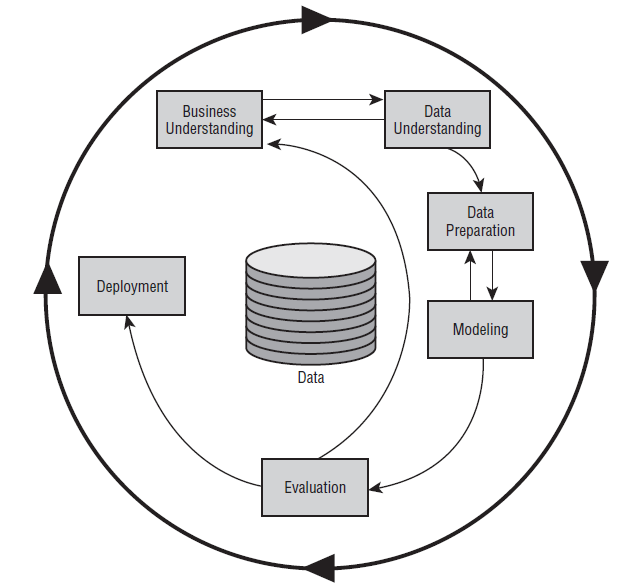
\includegraphics[scale=0.5]{Graphics/crisp-dm.png}
    \caption{CRISP-DM Process}
    \label{fig:crisp-dm}
\end{figure}
%This thesis will not adopt the complete process caused by the simple fact that a part of the methods are only for the business scope where this thesis is acting in scope of research.
\newline
\newline
\newline
This chapter will first \ref{Ch:2:Acquisition} have a macro view on the loan application process to point out the steps where our data will come from. %The goal is to have a real-world point of view on the collection process.%
Then, the first 3 phases of CHRISP-DM process are described in respect to the context of this thesis:
\begin{itemize}
    \item \textbf{Business Understanding }  
    \begin{itemize}
        \item Acquisition \ref{Ch:2:Acquisition} 
        % DATA Centered Approach, - Data driven
        \item Overview \ref{Ch:2:Overview} will discuss the macro view of the data and present insides collected by look up on it from the real-world point of view.
    \end{itemize}
    \item \textbf{Data Understanding }
        \begin{itemize}
            \item Feature Description \ref{Ch:2:FeatureDesc} provide a micro view on the available data: mention types of the features and describe the semantic.
            \item in Data Exploration \ref{Ch:2:Exploration} an  analysis of data is made by using of statistical \ref{Ch:2:SSummary} and visual \ref{Ch:2:VSummary} summary techniques, to explore data in order to bring important aspects of that data into focus. Moreover subchapter \ref{Ch:2:CorAn} expose correlated features damaging classification accuracy and data quality \ref{Ch:2:DataQuality} is dealing with inconsistent data.
        \end{itemize}
    \item \textbf{Data Preparation }
            \begin{itemize}
                \item Chapter Preprocessing \ref{Ch:2:Preprocessing} contain a composition of well researched data preparation approaches with the goal to increase the model performance. Dealing with missed/inconsistent data in \ref{Ch:2:MVI}, changing data representation to fit in the model is described in \ref{Ch:2:CTNT}. Then \ref{Ch:2:PCA} Principle Component Analysis (PCA) is applied, which is a typical statistical tool to reduce dimensions and rescale the features (give them the properties of a standard normal distribution).
        \end{itemize}
\end{itemize}

\section{Acquisition}\label{Ch:2:Acquisition}
The underlying data treated in this thesis contain information, collected during the credit enquiry process, briefly illustrated in figure \ref{fig:behav-data}. In course of the application the potential borrower provide his personal information by stepping through the application web-form. Moreover, most of the interactions with web-form elements, pressed keys or tracked time between actions is also implicitly collected. The figure \ref{fig:behav-data} show up an overview of data collecting.
The initial data used in this thesis is provided as a table. The engineering aspects regarding collecting and provisioning of the table are not part of this work and will not be discussed further. 

\begin{figure}[h]
    \centering
    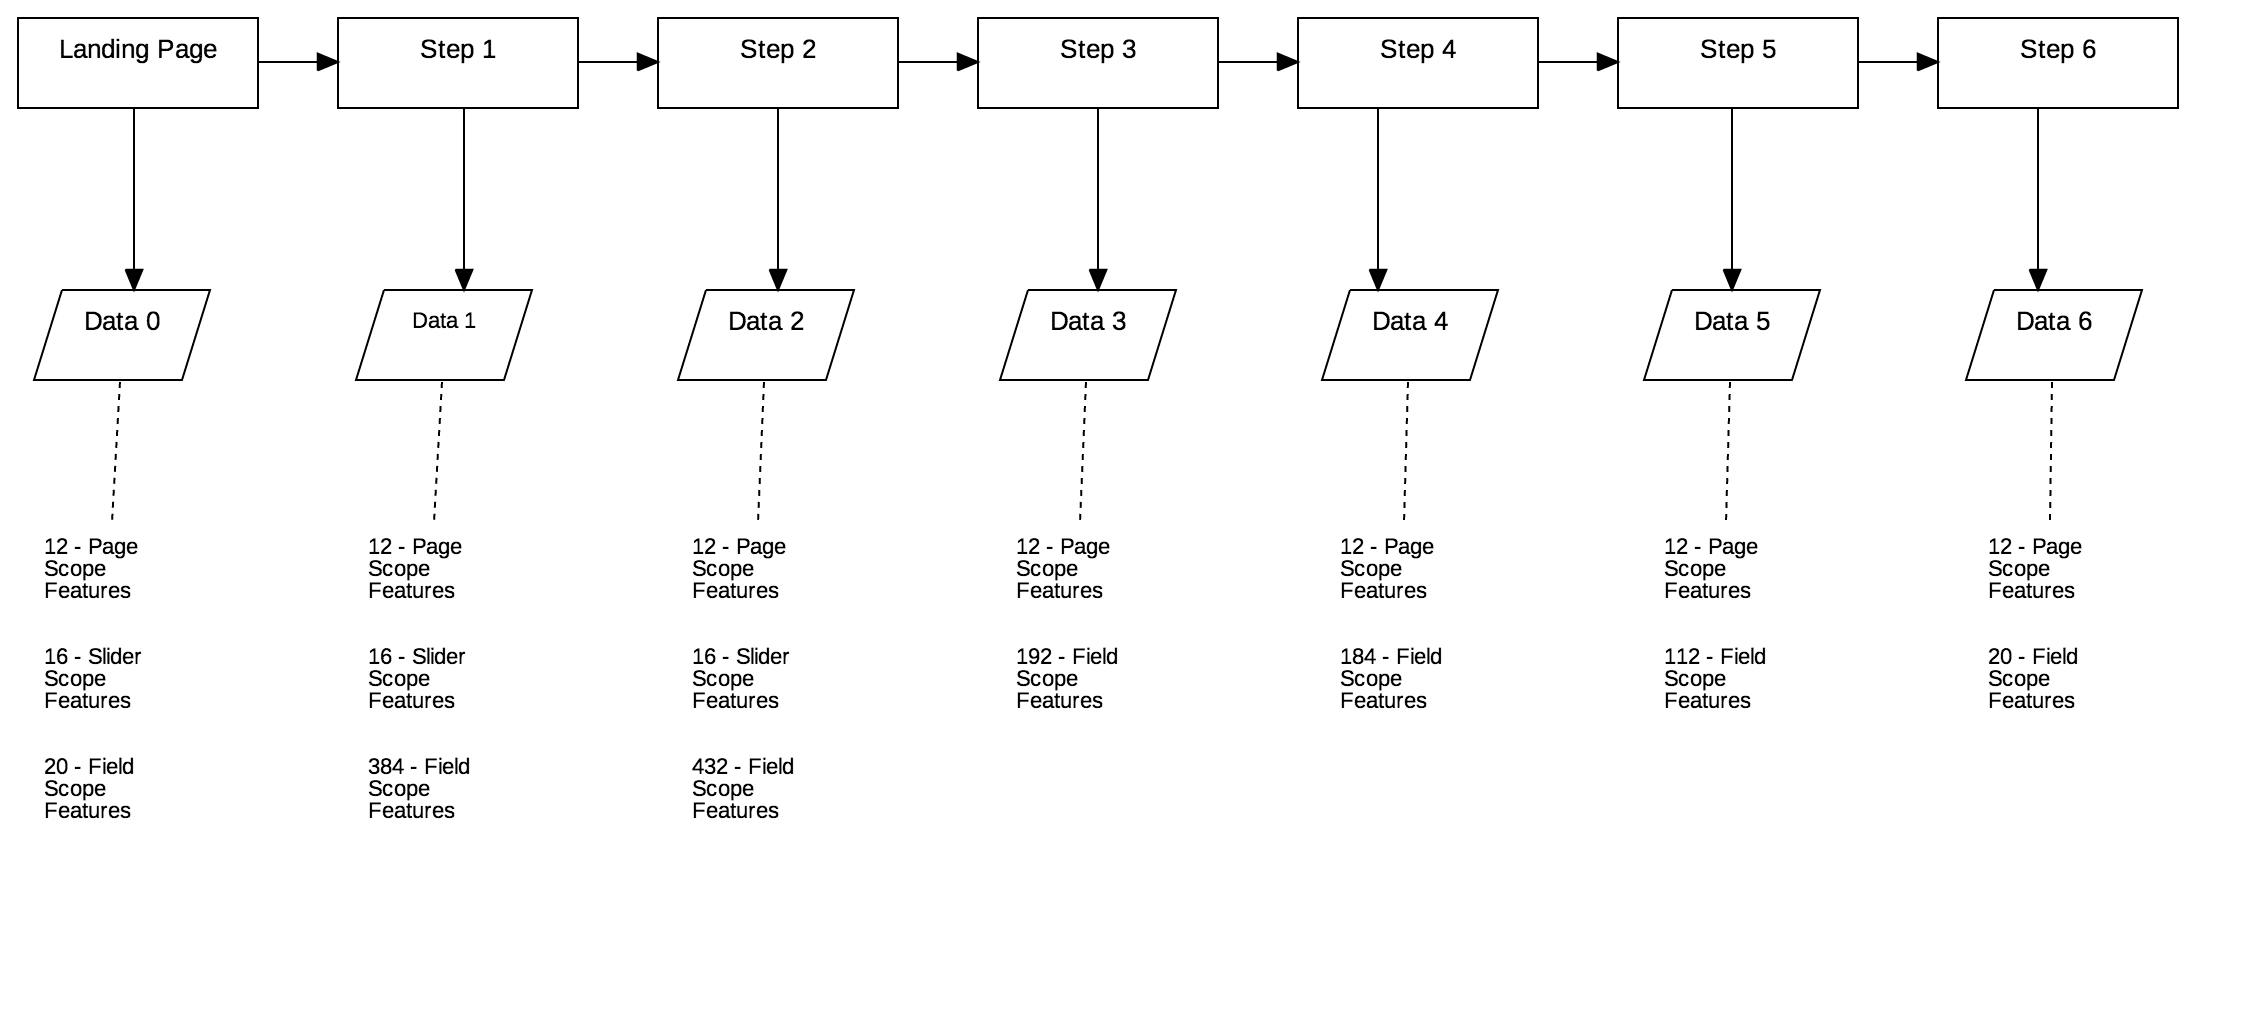
\includegraphics[scale=0.20]{Graphics/FlowchartDiagram1.png}
    \caption{Collection of Behavioral Data.}
    \label{fig:behav-data}
\end{figure}

The variables available are either categorical or numerical type and have two different sources:

\textbf{Variable Sources:}
\begin{itemize}
    \item User Input (Inputs made by the credit-applicant.)
    \item System Discovery (Variables that the application-system collect implicitly during the application-process.)
\end{itemize}

However, the variables from a scope of \textit{User Input} will be excluded from further analysis based on the fact that user inputs can be malicious. Although technical barriers are implemented, it is quite usual that fraudsters try to by-pass the process by inserting malicious information to receive a loan. This leads to the logical assumption that user generated input (such as monthly income, marital status, employee status etc.) is likely to contain intentionally false information. In comparison, the system collects continuous behavioral data \textit{Discovered by System} to detect fraudulent patterns in the course of the beginning to the end of the application process. Manipulation of behavioral information is significantly more difficult than inserting alternate personal information. The most obvious obstacle for the fraudster is to identify the technique and measures of behavioral assessment and this requires both technical experience and time which is usually not in relation to the benefits (small loan sizes). Considering these aspects, the following thesis is focusing on the behavioral data rather than the user input itself. 

\subsection{Overview (business understanding)}\label{Ch:2:Overview}

An effective utilization of data in machine learning requires a profound understanding of available data - also from a nontechnical perspective. In the following thesis, I will consider real-world aspects in which underlying data is potentially helpful for a solution.

Each data instance is representing information of an individual credit application, the information is historical and represents a common fact of a granted loan. This assortment is desirable. Granted means that this application have been approved by the scoring algorithm and the loan is issued to the borrower. Identifying anomalies signifying malicious actions in this type of data is of particular interest to prevent fraud in the future.

In following this Thesis introduce three assumptions to semantically structure (label) the available data for further algorithmic analysis.

\textbf{Fraud:} 
A small subset hold applications that in retrospect turned out to had fraudulent intention. This can have different causes, a portion has been reported by the local law enforcements, others are results of identity abuse or other malicious actions. This thesis will not amplify the fraud causes in detail and outline them simple as -  fraud.

\textbf{Non Fraud:} 
A borrower who payed at least one installment back is believed not to have any fraudulent intentions. 


\textbf{Unlabeled:}
A notable subset of underlying data contain application information not labeled as fraud but also not have positive cash flow, thus, this data can be classified as either fraud or nonfraud. 

\subsection{Feature Description}\label{Ch:2:FeatureDesc}

The underlying dataset contains in total 1804 features for each instance. All features are behavioral information which has been collected in the course of the credit application process (see: \ref{fig:behav-data}). An isolated description of each feature is not practical and thus not part of this Thesis. However, a more consolidated analysis is required. Table \ref{tab:feature-summary} summarize the data types contained in our data.


\begin{table}[h!]
  \begin{center}
    \caption{Feature type summary}
    \label{tab:feature-summary}
    \begin{tabular}{c|c|c}
    Type & Amount & Rate \\
      \hline
     Categorical & 196 & ~11\% \\ 
     \hline
     Logical & 90 &  ~5\% \\
     \hline
     Numeric & 1519 &  ~84\% \\
     \hline
    \end{tabular}
  \end{center}
\end{table}

Regarding to the figure \ref{fig:behav-data} there are 3 different scopes of behavioural features.

\begin{itemize}
    %write page on step chart
    \item \textbf{Page Scope:} Variables describing behavior in the scope of one of the 7 pages must be passed in credit application process. 
    \item \textbf{Slider Scope: } Variables in scope of an web-form element called \textit{slider}, it representing two interactive bars responsible for the adjusting of the loan amount the borrower apply for and the duration till the first installment.
    % rename to element scope
    \item \textbf{Field Scope:} Is the scope of all web form elements available through the enquiry process (input fields, buttons, check boxes, etc.).
\end{itemize}

Numerical features dominate the type distribution, in particular, most of them contain behavioral information e.g (count of keys been pressed by the user, time between interactions at input fields, etc.). Categorical features represent the types of web form elements triggered by user e.g (input field with text, drop down box with numbers, etc.). The remaining portion of logical fields containing boolean information (TRUE/FALSE) on questions regarding the behavior during the application e.g (did the user read the terms of the agreement?, did the user submitted his real email address on the first try? ... , etc.).

\section{Exploration}\label{Ch:2:Exploration}

This task addresses data mining questions using querying, visualization, and reporting techniques. These include distribution of key attributes (for example, the target attribute of a prediction task) relationships between pairs or small numbers of attributes, results of simple aggregations, properties of significant subpopulations, and simple statistical analyses. These analyses may directly address the data mining goals, they may also contribute to or refine the data description and quality reports, and feed into the transformation and other data preparation steps needed for further analysis \cite{crisp}.

\subsection{Statistical Summary of Data}\label{Ch:2:SSummary}

In total, our underlying data-set holds 95951 instances of individual applications.

According to the semantic labeling \ref{Ch:2:Overview} Table \ref{tab:instance-summary} summarize the amount of particular labels.

\begin{table}[h!]
  \begin{center}
    \caption{Instance Type Summary}
    \label{tab:instance-summary}
    \begin{tabular}{c|c|c}
    Label & Amount & Rate \\
      \hline
     Fraud & 744 & ~1\% \\ 
     \hline
     Nonfraud & 82525 &  ~86\% \\
     \hline
     Unlabeled & 12682 &  ~13\% \\
     \hline
    \end{tabular}
  \end{center}
\end{table}
It shows up that non-fraudulent instances clearly dominating the class membership where in the contrary the fraudulent representing a small subset. However, anomalies are rare by definition so this is a common pattern.

Summarizing over the category amount in categorical type features show up: 
\begin{itemize}
    \item \textbf{Min: } 2 Categories
    \item \textbf{Max: } 6 Categories
    \item \textbf{Mean:} 3 Categories
\end{itemize}
This observation is important insofar as each category adds a further dimension during the categorical to numerical transformation process \ref{Ch:2:CTNT}.
There are numerous well-known exploration techniques (like mathematical average, standard deviation or variance to name a few), unfortunately applying these on the high amount of features available would not necessary yield a valuable result. Based on this fact, further summary techniques are beyond the scopes and will not be considered.
\subsection{Visual Summary of Data}\label{Ch:2:VSummary} 
 
- Here  1-2 histograms of interesting variables, then explain that the complexity to show up everything is to high.

\subsection{Data Quality (missing values)}\label{Ch:2:DataQuality}
\epigraph{The only really good solution to the missing data problem is not to have any. Statistical adjustments can never make up for sloppy research. }{Paul D. Allison, 2001}
\label{intro}

Lack of information or missing data in a given data set is a common obstacle in field statistics and data mining. Investigations on the quality of data aim to identify lacks, which will benefit the desired machine learning algorithm. 

Bellow an descriptive analysis is made to identify the amount of missing data. Table \ref{tab:missings-over-all} present a statistical summary of missing rate in our source data.
 \begin{table}[h!]
  \begin{center}
    \caption{Summary of missing over the entire data.}
    \label{tab:missings-over-all}
    \begin{tabular}{c|c|c|c|c|c}
    Min & 1st Quartile & Max & Median & Mean & 3rd Quartile \\
      \hline
     0\% & 8\% & 99\% & 31\% & 43\% & 77\% \\ 
     \hline 
    \end{tabular}
  \end{center}
\end{table}

Since the lack of data is present, a deeper investigation is required. Missing data can have different types (in the context of statistical analysis). According to \cite{Allison:2007} there are three categories of missing data:

 \begin{itemize}
    \item \textbf{Missing Completely At Random (MCAR)} means that the probability of missing is unrelated to the variable itself or other variables. 
    \item \textbf{Missing At Random (MAR)} address missing in variables that is unrelated to itself. For example the probability of missing in income may depends on the employment status, but not depend on the income.
    \item \textbf{Not Missing At Random (NMAR)} eventuates when MAR is gone to be violated, ergo the probability of the missing depend on the particular value.
 \end{itemize}
 
Identifying the right category is important to select the correct treatment. However, classify the category of missing is not straight forward. An assumption about the membership is always based on observations on data and domain specific knowledge of data collection process.

Bellow missing amount is broken down to the summary on data grouped by type.

 \begin{table}[h!]
  \begin{center}
    \caption{Summary of missing over logical data.}
    \label{tab:missings-over-logical}
    \begin{tabular}{c|c|c|c|c|c}
    Min & 1st Quartile & Max & Median & Mean & 3rd Quartile \\
      \hline
     5\% & 9\% & 99\% & 31\% & 43\% & 76\% \\ 
     \hline 
    \end{tabular}
  \end{center}
\end{table}
 
 \begin{table}[h!]
  \begin{center}
    \caption{Summary of missing over numeric data.}
    \label{tab:missings-over-numeric}
    \begin{tabular}{c|c|c|c|c|c}
    Min & 1st Quartile & Max & Median & Mean & 3rd Quartile \\
      \hline
     0\% & 8\% & 99\% & 30\% & 41\% & 76\% \\ 
     \hline 
    \end{tabular}
  \end{center}
\end{table}
   

 \begin{table}[h!]
  \begin{center}
    \caption{Summary of missing over categorical data.}
    \label{tab:missings-over-categorical}
    \begin{tabular}{c|c|c|c|c|c}
    Min & 1st Quartile & Max & Median & Mean & 3rd Quartile \\
      \hline
     0\% & 24\% & 99\% & 59\% & 58\% & 90\% \\ 
     \hline 
    \end{tabular}
  \end{center}
\end{table}


Analytics done on missing amount of numerical \ref{tab:missings-over-numeric}, logical \ref{tab:missings-over-logical} and categorical \ref{tab:missings-over-categorical} types, show up that no type is gapless of lacks. The statistics over missings in logical and numeric data are quite similar, this fact can lead to the assumption that the causes of lacks can be related to a common factor(s). This, in turn, is indicative to MAR category of missing.

A common technique to build an assumption about the category of missing is to inspect so called \textit{missing patterns}. It contributes to understanding whether groups of variables tend to be either all missing or all observed. Table \ref{tab:variable-pattern-example} present a matrix, in which each row corresponds to a missing data pattern \textit{(1=observed, 0=missing).} 

\begin{table}[h!]
\centering
\caption{Missing pattern applied on four random variables.}
\label{tab:variable-pattern-example}
\begin{tabular}{lllll}
\textbf{Amount} & V1 & V2 & V3 & V4 \\
901             & 1           & 1           & 1           & 1           \\
20              & 1           & 1           & 0           & 1           \\
4510            & 1           & 1           & 1           & 0           \\
2               & 0           & 1           & 1           & 1           \\
6               & 1           & 0           & 1           & 1           \\
87847           & 1           & 1           & 0           & 0           \\
9               & 0           & 1           & 1           & 0           \\
55              & 1           & 0           & 0           & 1           \\
6               & 1           & 0           & 1           & 0           \\
572             & 0           & 1           & 0           & 0           \\
716             & 1           & 0           & 0           & 0           \\
1307            & 0           & 0           & 0           & 0          
\end{tabular}
\end{table}

Furthermore, there is a visual investigation approach to identify missing patterns. Figure \ref{fig:missing-plot} present two plots. The histogram shows up the rate of missing values and the box plot is the visualisation of missing patterns.

\begin{figure}[h!]
    \centering
    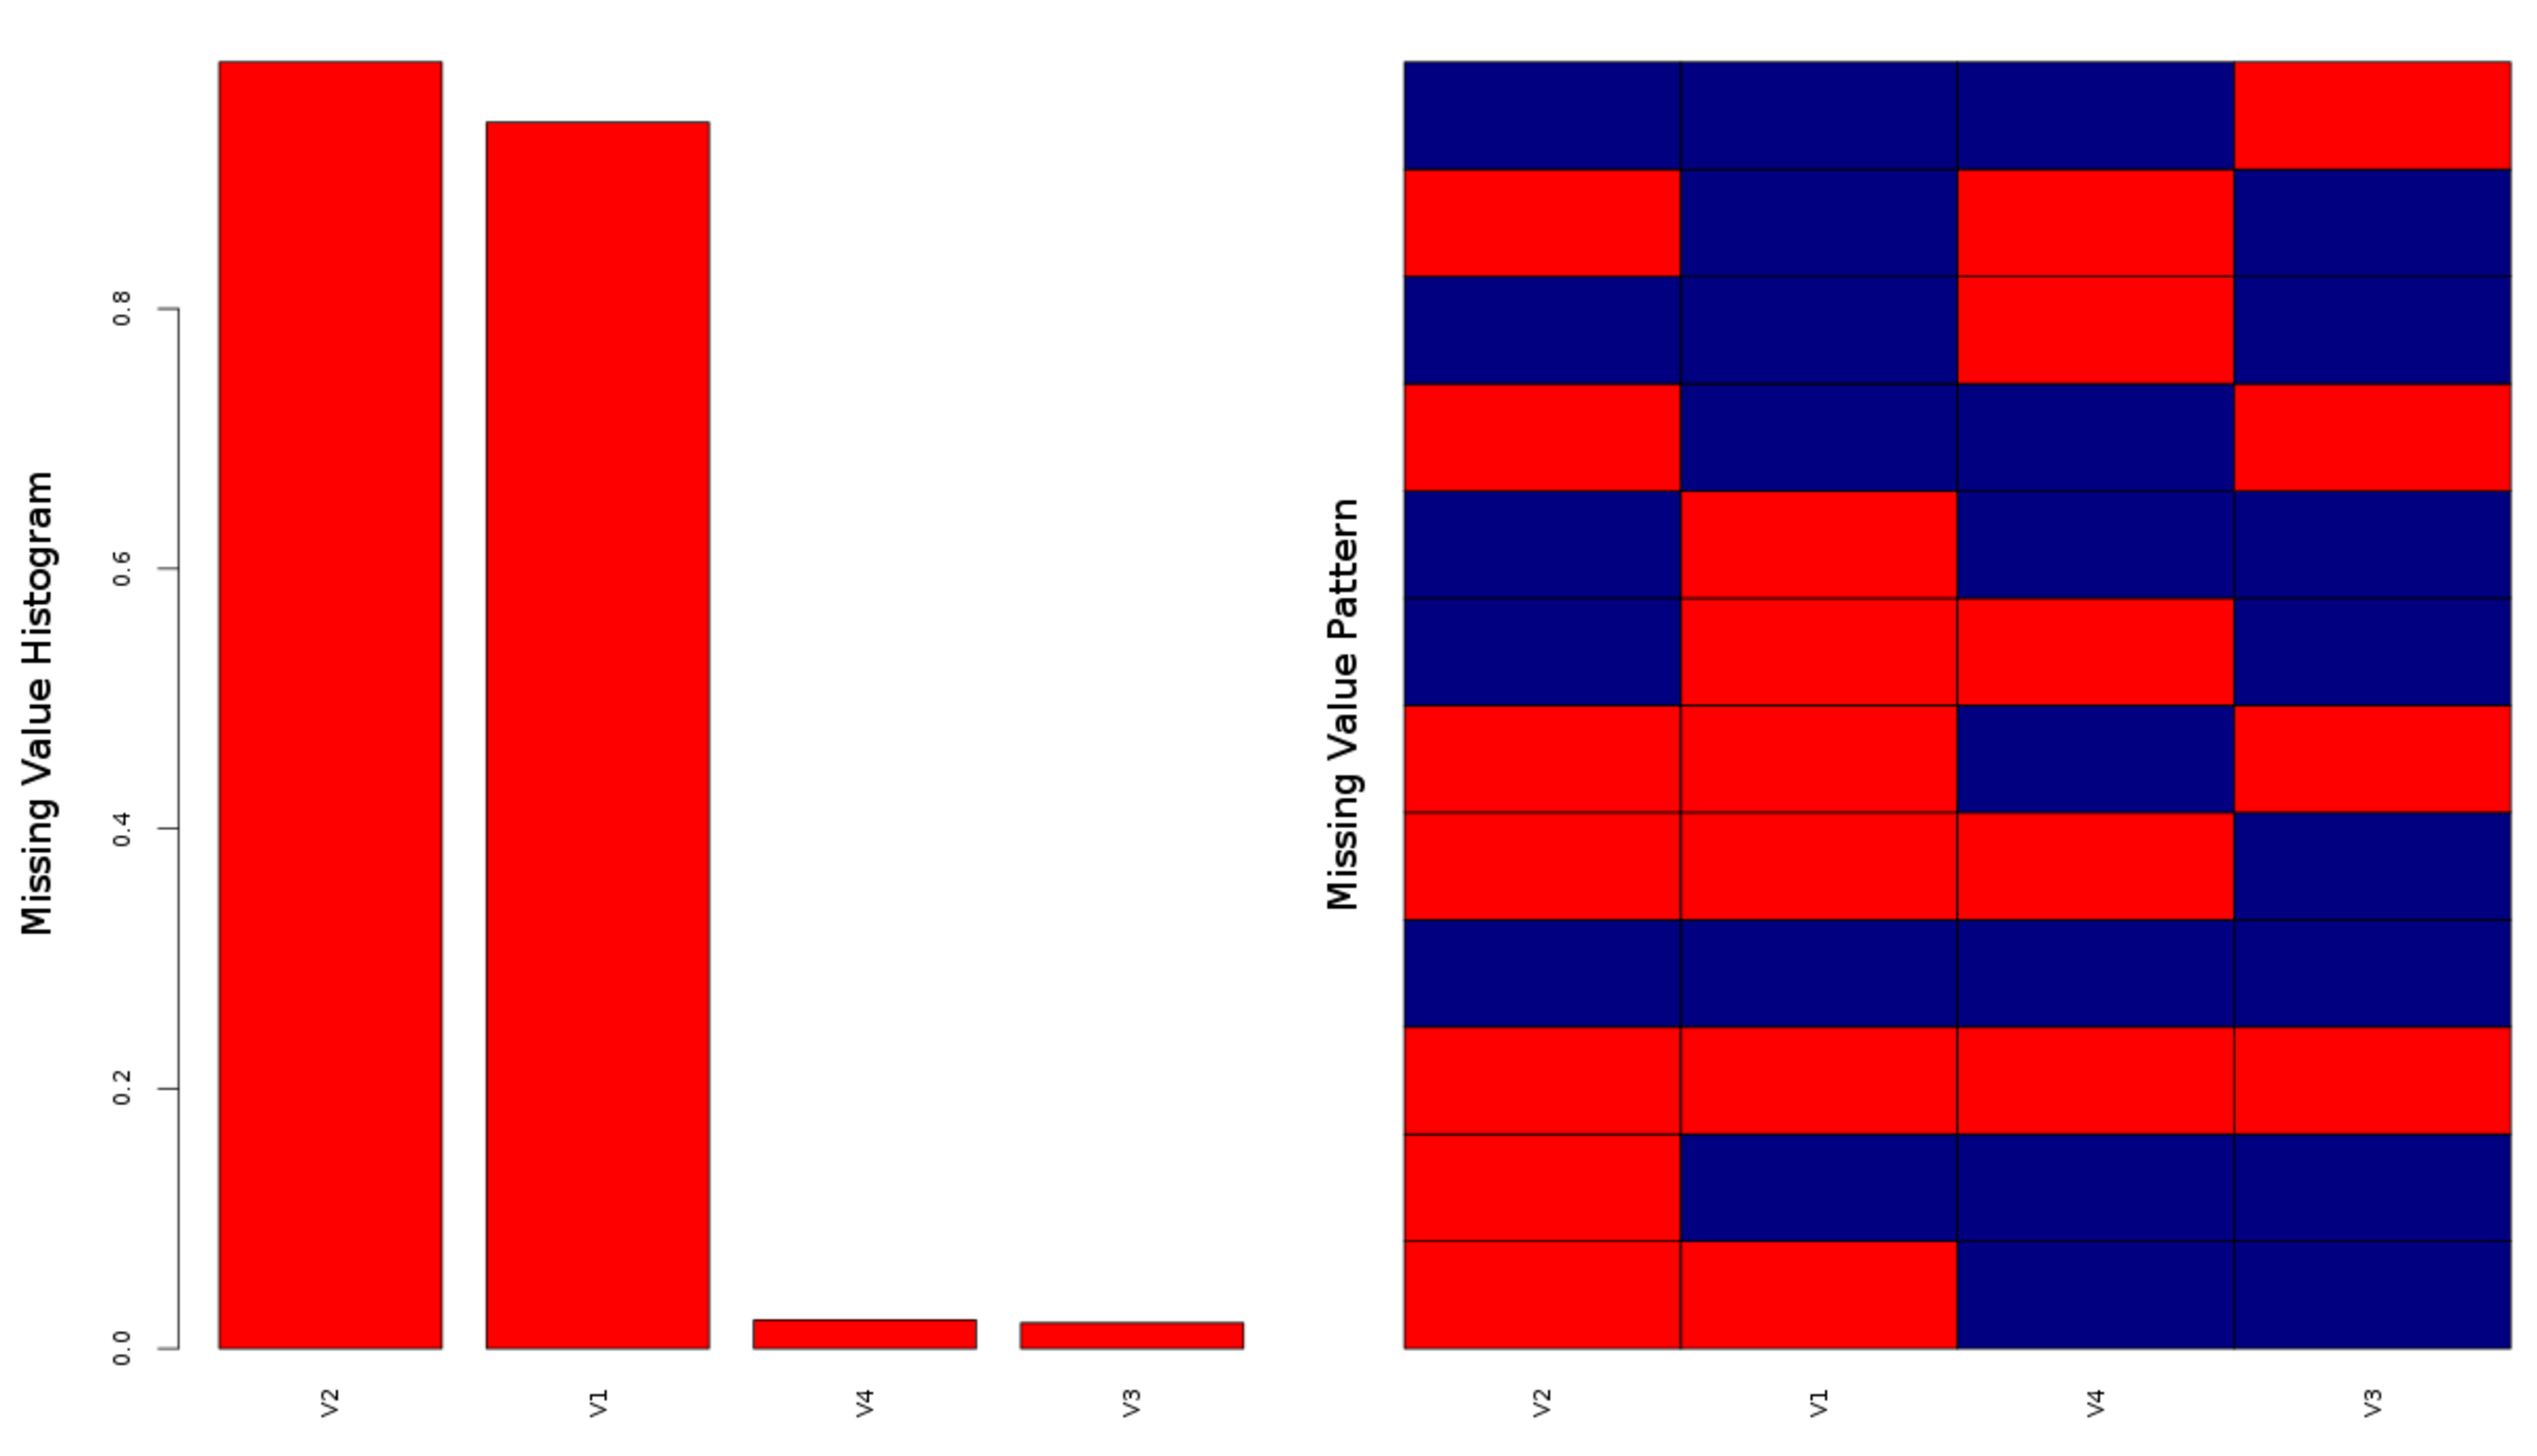
\includegraphics[scale=0.3]{Graphics/missing-pattern-plot.png}
    \caption{Plot possible patterns of missing data.}
    \label{fig:missing-plot}
\end{figure}

Unfortunately, these methods of analysis not fitting well with our amount of features. A pattern matrix describing all possible patterns on data given in this thesis would be obviously hard to manage. Pattern analysis can also be applied to a subset of data - to yield more coherent results, However, the creation of the suitable subset efforts an assumption to chose the suspicious features.

It is conceivable, that more advanced analytics would produce valuable results in the case of missingness classification. However, this topic would deserve a separate research paper and exceed the scope of this thesis. Furthermore, the interested reader is referred to the work of \cite{Mohan;Pearl:2014} where a promising approach for Testability of missing category is provided.

As last but not least, initial improving data quality should also be considered. Possible causes of missing values can be a helpful information to start with quality treatment. 
Potential causes could be:
    \begin{itemize}
    
        \item Behavior data is describing several interactions with web form components, some of them are optional.
        
        \item Application data is obviously processed through several instances before it is available for data analysis. The processing and data conversions related to this process could be responsible for the loss of data.
        
        \item The credit application process was executed by a non-human but so-called script/bot \footnote{A bot (short for "robot") is a program that operates as an agent for a user or another program or simulates a human activity on the Internet. (http://searchsoa.techtarget.com/definition/bot)}. A bot obviously skips the most of the interactions a human would have to do during the application. 
    
        \item The particular operation system on top the application is executed can be modified to block the gathering of information by the application system.
    \end{itemize}


\section{Preprocessing}\label{Ch:2:Preprocessing}
Based on the observations obtained through acquisition and exploration of our data, this section will explain the explicit steps of data transformation made before fitting it in our model.

\subsection{Missing Value Imputation}\label{Ch:2:MVI} 
  IN PROGRESS (To Liuben: already imputed everything as median, i will reason it with the easiest method, please leave a short note if you agree or not and why :))
 
\subsection{Categorical to Numeric Transformation}
\label{Ch:2:CTNT}
The most of the statistical learning algorithms like them provided in this thesis (chapter: \ref{ch:3}), can't deal with other than numerical data types. Since the analysis of a number of types contained in our data \ref{tab:feature-summary}, is known that beside numerical also categorical and logical types are components of given feature set. 

Thus, a number of nonnumerical features are not minor, the utilization of these can have a significant impact on model accuracy. A common approach to convert categorical values into numerical representation is binarization where each value is transformed in either 1 or 0.

Let us consider a categorical feature \textit{action} describing the input behavior happened to process the next step during the credit inquiry, the possible categories were given: 


\[ \{ButtonClick, MouseClick, Other\} \]

For the sake of simplicity we consider a subset with only four instances see table \ref{tab:feature-categorical-rep} for an example representation. 

\begin{table}[h!]
  \begin{center}
    \caption{Example of categorical representation.}
    \label{tab:feature-categorical-rep}
    \begin{tabular}{c|c}
    instance & action \\
      \hline
     A & Other \\ 
     \hline 
       B & MouseClick \\ 
     \hline
       C & ButtonClick \\ 
     \hline
       D & Other \\ 
     \hline
    \end{tabular}
  \end{center}
\end{table}

Applying the binarization on these would yield three additional features with an numerical value of either \(1\) or \(0\). Table \ref{tab:feature-binarization} illustrates the view after binarization.

\begin{table}[h!]
  \begin{center}
    \caption{Example of feature binarization.}
    \label{tab:feature-binarization}
    \begin{tabular}{c|c|c|c|}
    instance & action.ButtonClick & action.MouseClick & action.Other \\
      \hline
     A & 0 & 0 & 1 \\ 
     \hline 
       B & 0 & 1 & 0 \\ 
     \hline
       C & 1 & 0 & 0 \\ 
     \hline
       D & 0 & 0 & 1 \\ 
     \hline
    \end{tabular}
  \end{center}
\end{table}

However, each possible category adds another feature ergo another dimension to the underlying data set, it should be considered that high amount of dimensions have several side effects like increasing computation time or noise.

\subsection{Removing (near) Zero Variance Features}\label{Ch:2:RNZVF}
After the quality of data is been treated its time to care about reducing model complexity. Removing of predictors with zero and near zero variance is a typical preprocessing technique used for dimension reduction. 

Observations made by inspecting the data quality \ref{Ch:2:DataQuality} showed up  a non-inconsiderable amount of missing values, this fact leads to the assumption that our underlying data could be contaminated with low and zero variance features.

\textbf{Zero variance:} stands basically for statistical variance is zero, so the predictor is a constant.

\textbf{Near zero variance:} is more complex and means to identify  variables with a low unique value rate - relative to the number of samples or have a large ratio of the most common value in respect to the second most common value.

Summarized it can be said that removing can drastically reduce the computation time and also increase model accuracy by doing dimension reduction. However, removing it is not necessary always the best way, for example, an binary feature with lots of zeroes and few ones could be an legit indicative for class membership but the near zero variance process would possibly remove it.

Another considerable aspect is that normally the historical data is growing with the time - so, the probability that the variance will change is given.

\subsection{Principle Component Analysis (PCA)}\label{Ch:2:PCA} 
Principle Component Analysis is one of the main methods to reduce dimensionality, first introduced by Karl Pearson \cite{Pearson:1901}. The main idea behind PCA is to find patterns by identifying high correlated feature and remove them - dimensionality decreasing. The leftovers are the maximal variance components that contain the most information.  

The analysis made in chapter \ref{Ch:2:FeatureDesc}, showed up a lot of features contained in the underlying dataset, moreover the transformation of categorical and logical to numerical features \ref{Ch:2:CTNT} will extend the feature size. Based on the fact of large feature space and on experiments already done combining classification algorithms and dimensionality reduction \cite{5446692}, doing PCA is a reasonable process to help improve the discriminative power of classifiers.

Formally, the goal of PCA is to produce given examples from higher to lower space:

\[ x \in X \in {\rm I\!R}^n \textrm{ to } z \in Z \in {\rm I\!R}^k \]
\[ \textrm{where } k \leq n \]

The classical approach is first to compute a \(n \times n \) covariance matrix, where each element is the covariance between two features:

\[ \Sigma = \frac{1}{m}\sum_{i = 1}^{n}(x^i)(x^i)^T\]
\[ \textrm{where }(x^i) \textit{ is an } (1 \times n) \textrm{ vector and } (x^i)^T \textrm{is an } (n \times 1) \textrm{ vector.}\]

Based on the result of the covariance matrix, eigenvectors should be computed. Eigenvectors determine the direction of new feature space and their eigenvalue explain the variance of the data.
There are several methods to figure out the eigenvectors, in this thesis \textit{Singular Value Decomposition} (SVD) will be used, which is known to be rather numerical stable than the native one method called \textit{eigendecomposition}. 

Applying SVD on the covariance matrix, yield:

\[ [U,S,V] = SVD(\Sigma)\]
\[ \textrm{where  } U \in  {\rm I\!R}^{n \times n} \textrm{ Matrix representing the eigenvectors.}  \]

Sorting eigenvalues of the given eigenvectors and choosing the \( k \) count corresponding to the largest eigenvalues, will result in \( U' \in   {\rm I\!R}^{n \times k}\) matrix.
Transforming the original data \( X \) to the projection \( Z \) by:

\[ Z = X U'^ T \]
finally makes the deal to transform initial data to k-dimensional feature subspace.

Nonetheless, dimensionality reduction is always an act of information loss, so the fact that PCA can also hurt classification accuracy should be considered. Moreover, several methods for dimensionality reduction were compared in combination with classification algorithms and showed partially better results than PCA \cite{Cao2003321}. 
\chapter{Machine Learning Methods}\label{ch:3}
This chapter will treat the machine learning methods applied in this thesis. The subsection Support Vector Machines: \ref{Chapter:SVM}, will point out the idea of SVM including an introduction into the theoretical parts. Followed by: \ref{Chapter:PUL} where the Positive Unlabeled Learning (PUL) strategy for \textit{training} of our prediction model is discussed. The subjecting chapter: \ref{Chapter:OC-SVM} approach on One Class SVM, it will cover the concept and the gaps in respect to the ordinary SVM. At the end of this chapter, the subsection: \ref{Chapter:Ensemble} will introduce the concept of Ensembles in the scope of machine learning especially to improve the classification accuracy.

The purpose of the following introduction is:
\begin{itemize}
    \item Understand the core concept of the particular algorithms.
    
    \item Get a brief understanding of the theoretical concepts driving the algorithms.
    
    \item Became familiar with the possible tuning options that the algorithms contain and be able to track the motivation of adjusting them.
\end{itemize}
One last note before starting: the theoretical concepts will be presented in an aggregated form. The goal is to provide only the information necessary to follow up in the further chapter. 


\section[Support Vector Machines (SVM)] {Support Vector Machines (SVM) \footnote{The following chapter is based on the chapter 8 of the book \textit{Applications of Supervised and Unsupervised Ensemble Methods} by \cite{Okun;Valentini:2009}, and provide a brief summary of SVM important for further work in this Thesis. } }\label{Chapter:SVM}

%http://stats.stackexchange.com/questions/63028/one-class-svm-vs-exemplar-svm
Support Vector Machines (SVM) \cite{Cortes;Vapnik:1995} is a state-of-the-art method with a solid background in statistical learning theory. It can be used for both classification and regression tasks. What distinguishes an SVM from other methods is a better ability to deal with high dimensional data and the guarantee of the globally optimal solution. The solution an SVM produces is sparse in many cases as only a fraction of training set instances is relevant for the task at hand. These instances, called support vectors, lie close to a hyperplane separating data into classes. Thus, an SVM tries to transform nonlinearly separable classes into linearly separable ones because the latter case is simpler to solve than the former. Without loss of generality and for the purpose of this thesis, only one or two classes are assumed to be present in the data.

Let us assume that we are given a data set as
\[  S = \{(x_1,y_2), (x_2,y_2), ...,(x_n,y_n) \} \; x_i \in \mathbf{R^d} \; y_i \in \{-1,1\}, \]
where \( x_i\) is the \( i-\)th input instance or data point and \( y_i\) is its class label. Thus, \(x_i\) is a \(d-\) dimensional column vector whereas \( y_i\) is a scalar.

A hyperplane that splits the data into two classes can be represented with the following equation:
\[\vec{w}^Tx + b = 0, \] 
where \(\vec{w}\) is a \textit{weight vector} determining the direction perpendicular to the hyperplane and \(b\) a \textit{bias} responsible for moving the hyperplane parallel to itself (see also~\ref{fig:hyperplane1}).

\begin{figure}[h!]
    \centering % Picture from Oleg's book, do not forget the reffs!
    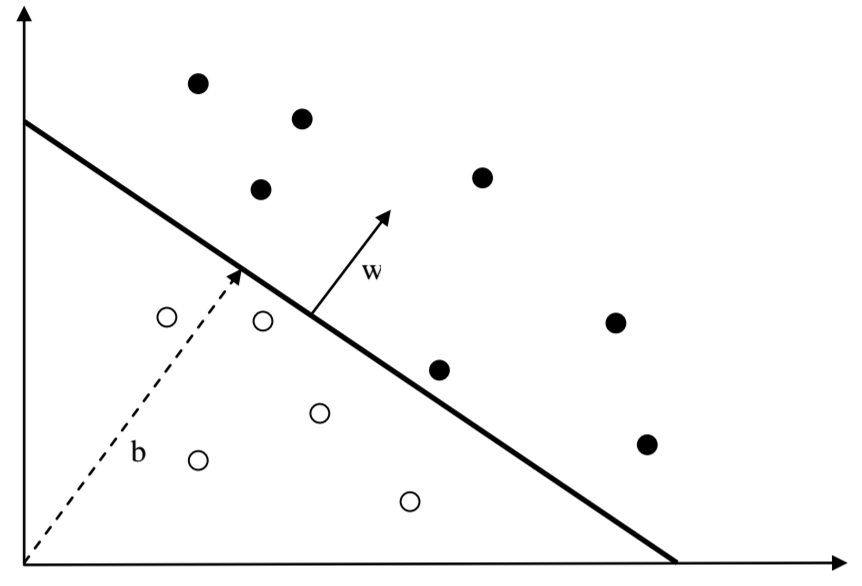
\includegraphics[scale=0.6]{Graphics/svm1.png}
    \caption{Hyperplane for separating 2-dimensional data.}
    \label{fig:hyperplane1}
\end{figure}

However, classes in the input space are often not linearly separable, which means that a linear classifier is not a good option in such a case. In the case of SVMs a solution is to project the original data into another, often a higher dimensional space \(x \mapsto \phi(x) \), where classes would more likely be linearly separable. Figure~\ref{fig:hyperplane2} shows an example of input space \(X\) where data cannot be separated by a linear function. However after applying the mapping function \(\phi\) to each data point in \(X\), the data become well separable in a \textit{feature space} \(F = \{ \phi(x)\; | \; x \in X\}\).
\begin{figure}[h!]
    \centering
    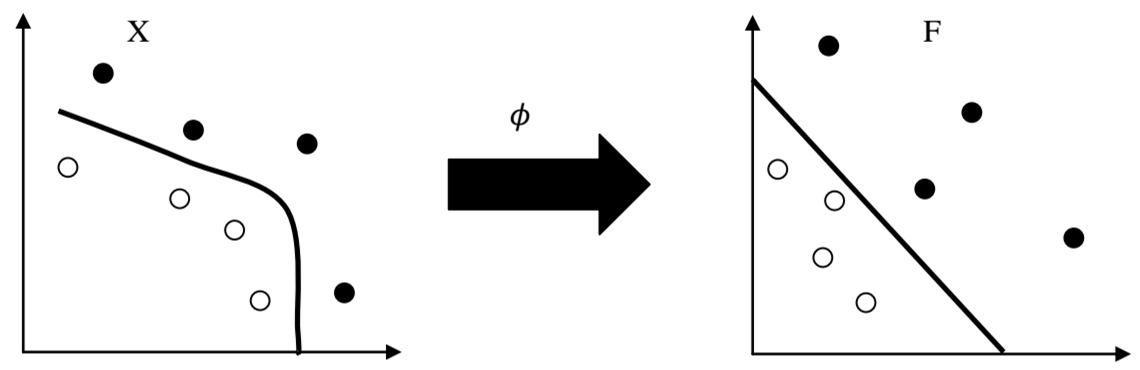
\includegraphics[scale=0.6]{Graphics/svp-separation.png}
    \caption{Mapping data into feature space.}
    \label{fig:hyperplane2}
\end{figure}

Thus, a straightforward solution seems to transforms data into a feature space where a linear classifier can be built. These two operations are combined with the help of a kernel function. The typical kernel functions are:
\begin{itemize}
            \item \(K(x,z) = x'z \) - linear kernel
            \item \(K(x,z) = (\tau + x'z)^p\) - polynomial kernel of degree p
            \item \(K(x,z) = exp(-\sigma||x-z||^2)\) - Gaussian or Radial Basis Function (RBF) kernel
\end{itemize}

In these definitions, only $x$ and $z$ are vectors while other symbols denote scalars.

As one can see, the kernel representation eliminates the necessity to map each input individually: the inputs never appear isolated but in the form of inner products between pairs of vectors. Because of this, we don't need to know the underlying feature map! Also, the dimensionality of the feature space does not affect the computation as the inner product is a number. As a result, the only information that is necessary is a \(n\times n\) kernel matrix.

Kernels provide one pillar of SVMs. The other is the optimization theory as the SVM solution is formulated as an optimization task, subject to certain constraints. The primal optimization problem where \( w \) and \( b \) are involved is difficult to solve due to inequality constraints. Instead, the dual problem based on  Lagrangian theory \footnote{Lagrangian theory is a basic mathematical tool for constrained optimization of differentiable functions, especially for nonlinear constrained optimization \cite{Li:2008}.} transforms the task into a quadratic program where the function to be optimized is quadratic while the constraints are all equalities rather than inequalities. The solution of such a problem is known to be unique and global. It is also sparse by implying that only a small fraction of the original data matters for class separation, which results in a very efficient classifier.

Below both primal and dual optimization problems are given. The maximal (or hard) margin problem assumes two classes are only linearly separable in the feature space. To remedy its deficiency, the soft margin problem is then presented that works with nonlinearly separable classes by introducing slack variables measuring non-separability (see below).

The margin is a quantity indicating how well two classes of data are linearly separable. Figure~\ref{fig:hyperplane3} shows the maximal margin $\gamma$ for a set of 2D points. Thus, the margin is a half distance between two hyperplanes parallel the class-separating hyperplane when this separation is maximized.
\begin{figure}[h!]
    \centering
    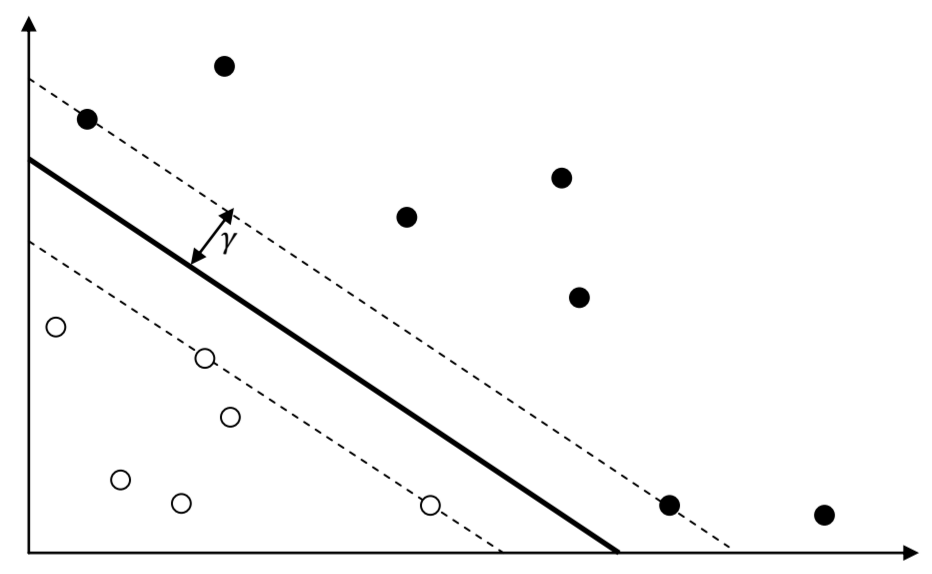
\includegraphics[scale=0.6]{Graphics/svm-margins.png}
    \caption{The margin of a set of points.}
    \label{fig:hyperplane3}
\end{figure}

\textbf{The maximal margin:}

\[\textrm{Primal problem:}\; \textrm{minimize}\; \vec{w} \vec{w},\] \[\textrm{subject to:}\; y_i(\vec{w}\vec{x_i} + b) \geq 1, i = 1, ...,l \] 

\[\textrm{Dual problem:}\; \textrm{maximize}\; W(a) =  \sum_{i=1}^{l} a_i - \frac{1}{2}\sum_{i,j = 1}^{l}a_i a_j y_i y_j K(\vec{x_i}^T \vec{x_j}), \] 
\[\textrm{subject to:}\; \sum_{i=1}^{l}a_i y_i = 0, a_i \geq 0, i = 1,...,l.\] 

\textbf{The 2-norm soft margin:}

\[\textrm{Primal problem:}\; \textrm{minimize}\; \vec{w} \vec{w} + C \sum_{i=1}^{l} \xi^2_i\; \textrm{over}\; \xi,\vec{w},b\] 
\[\textrm{subject to:}\; y_i(\vec{w}\vec{x_i} + b) \geq 1 - \xi_i,, i = 1, ...,l \] 

\[\textrm{Dual problem:}\; \textrm{maximize}\; W(a) =  \sum_{i=1}^{l} a_i - \frac{1}{2}\sum_{i,j = 1}^{l}a_i a_j y_i y_j \Big( K(\vec{x_i}^T \vec{x_j}) + \frac{1}{c}\delta_i \Big), \] 
\[\textrm{subject to:}\; \sum_{i=1}^{l}a_i y_i = 0, a_i \geq 0, i = 1,...,l.\] 

\textbf{The 1-norm soft margin:}

\[\textrm{Primal problem:}\; \textrm{minimize}\; \vec{w} \vec{w} + C \sum_{i=1}^{l} \xi_i\; \textrm{over}\; \xi,\vec{w},b\] 
\[\textrm{subject to}\; y_i(\vec{w}\vec{x_i} + b) \geq 1 - \xi_i,\xi_i \geq 0, i = 1, ...,l.\] 

\[\textrm{Dual problem:}\; \textrm{maximize}\; W(a) =  \sum_{i=1}^{l} a_i - \frac{1}{2}\sum_{i,j = 1}^{l}a_i a_j y_i y_j K(\vec{x_i}^T \vec{x_j}) , \]
\[\textrm{subject to}\; \sum_{i=1}^{l}a_i y_i = 0,C \geq a_i \geq 0, i = 1,...,l.\] 

\subsection{One Class SVM}\label{Chapter:OC-SVM}
\textit{One Class SVM} is an SVM-based classifier method proposed for cases when only one class of data is available to a modeler. Another important distinction from the conventional SVM is that instead of the separating hyperplane a hypersphere with minimal volume (or
minimal radius) containing all objects is sought \cite{Tax:2004:SVD:960091.960109}. 

As can be seen in the figure: \ref{fig:hypersphere} \footnote{The picture is taken from the work of  \cite{s120810109}}, everything inside the sphere describes instances of a given class where outside lie outliers. 

\begin{figure}[h!]
    \centering
    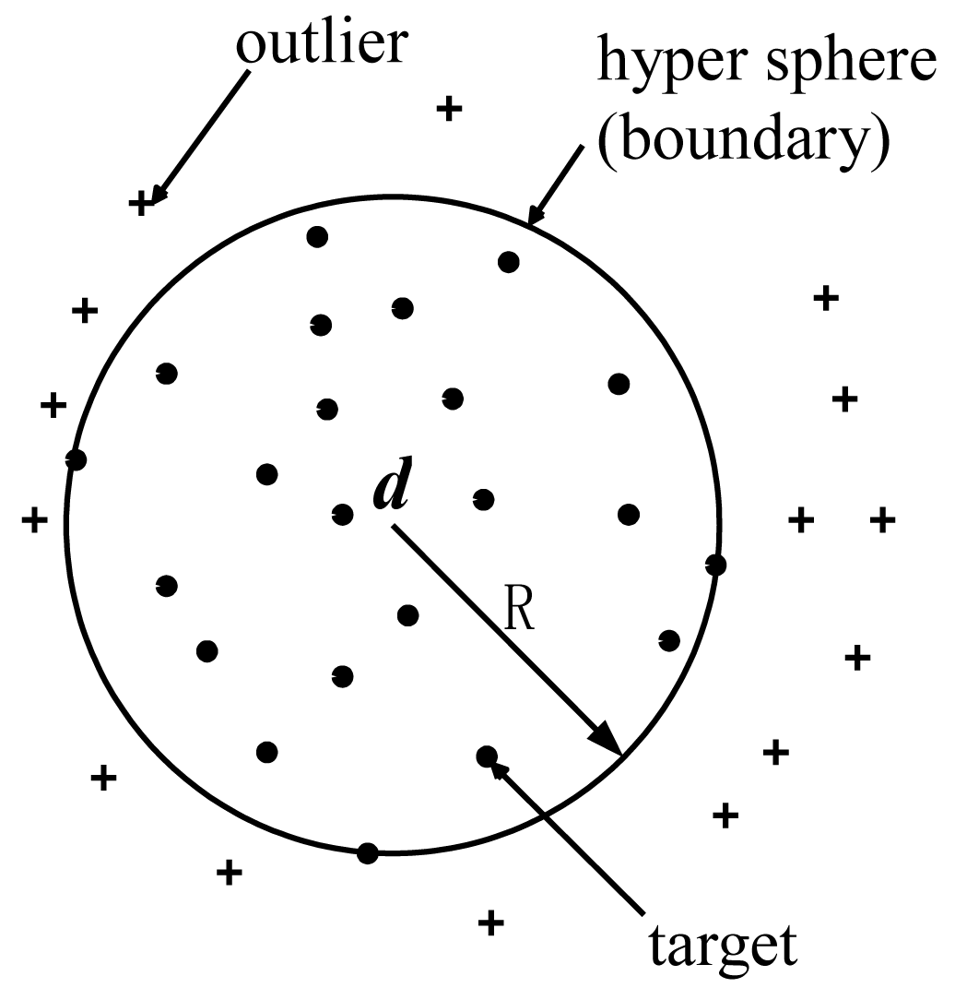
\includegraphics[scale=0.2]{Graphics/tax-duin-svm.png}
    \caption{One class classification with Support Vector Data Description by \cite{Tax:2004:SVD:960091.960109}.}
    \label{fig:hypersphere}
\end{figure}

The resulting hypersphere is described by center \(d\) and radius
\(R\). Bellow the optimization problem is given: 

\[ \textrm{Minimize } R^2 + C \sum_{i=1}^{n} \xi_i, \]
\[ \textrm{subject to: } || x_i - d ||^2 \leq R^2 + \xi_i, \textrm{ } \xi_i \geq 0, \textrm{ } i = 1, ..., n \]

Where \( \xi \) are the slack variables for soft margin optimization and \( C \)  is the penalty parameter that gives the trade-off between the volume of the sphere and the number of errors.

\section[Positive and Unlabeled Learning]{Positive and Unlabeled Learning\footnote{The description and formulas of the Positive and Unlabeled Learning algorithm in this chapter are based on the work of \cite{Elkan;Noto:2008}.}}\label{Chapter:PUL}

Positive Unlabeled Learning (PUL) is an approach on the \textit{learning a classifier from positive and unlabeled data} problem. Because only one class is available (positive), PUL could be considered as a kind of one-class task. However, using unlabeled data, which are plenty, given modern data collection technologies, turns this task into two-class classification. Unlabeled data are assumed to contain both positive and negative instances but their labels are unknown to an observer. Because in PUL settings the amount of one class of data often far exceeds the amount of the other class, the classification problem becomes imbalanced. One of the ways to solve class imbalance is to use cost-sensitive learning where errors made on different classes have different costs.

The goal of the PUL technique by \cite{Elkan;Noto:2008} is to learn the true function \(f(.)\) that can predict the positive \(P\) examples as closely as possible, by learning another function \(g(.)\) from positive and unlabeled \(U\) data. Also a validation set, separate from the training data, is needed in order to find a normalizing constant \(c\) for \(g(.)\). After that, given a test (unseen) vector \(x\), \(f(x)\) is found as \(g(x)/c\).

PUL pseudocode is given below: \ref{alg:PUL}. 

\begin{algorithm}[h!]                      
\caption{PUL by using SVM.} 
\label{alg:PUL}                          
    \begin{algorithmic}[1]
        \State $ D\gets P \cup U$ \Comment{Positive and Unlabeled data, where Unlabeled is implicitly a label.}
        \State $\{Train,Valid,Test\}\gets split(D)$ \Comment{Split the original data into training, validation, and test sets.}
        \State $g \gets svm(Train)$ \Comment{Train a cost-sensitive 2-class SVM.}
        \State $Prob = g(Valid)$ \Comment{Get probabilities of being positive for positive instances of the validation set.}
        \State $c = mean(Prob)$ \Comment{Calculate the normalizing constant as the mean probability.} 
        \State $Prob = g(Test) / c$ \Comment{Compute the probability of being positive for test data.}
        \State If this probability is larger than 0.5, label a test instance as positive
   \end{algorithmic}
\end{algorithm}

There the data is first divided into training, validation, and test sets. Then a cost-sensitive SVM is used to train a classifier, able to predict the probability of an instance being positive. The result of applying the classifier on the validation set yields the normalizing constant (by taking the mean probability) that is then used for generating test set predictions.

In other works on PUL, experimental results showed that this approach significantly reduces the effort of labeling the data, while yielding competitive results, compared to the case when both positive and negative labels must be known before learning (see \cite{Li:2011}).

\section{Ensemble SVM}\label{Chapter:Ensemble}
\textit{Ensamble SVM} is an approach to combine multiple SVM Algorithms. The general idea of sequential ensembles is to provide a better understanding of the data, so as to enable a more refined execution with either a modified algorithm or data set \cite{Aggarwal:2013} by applying the same or several classification algorithms on the same data and evaluating the results. Alternatively, independent ensembles use different initialisations of same algorithm or different subsets of underlying data. The results can be combined to obtain a more robust outlier score \cite{Aggarwal:2013}. 

This Thesis will stick on the Robust Ensemble of Support Vector Machine algorithm \cite{Claesen:2014} which can be defined as an independent ensemble.

The problem of PU learning can be considered as a supervised task with label noise in the negative set \cite{Claesen:2014}. However, the assumption that only the negative set can contain label noise can be violated due to various reasons \cite{journals/tnn/FrenayV14}. For example, our assumption that borrowers which have already paid at least one installment back are believed to not have fraudulent intentions (see Chapter ~\ref{Ch:2:Overview}), could be violated by making the assumption that some borrowers are paying a small installment back to hide their fraudulent intentions - that would mean those positive examples \(P\) can contain label noise.

Robust Ensemble of Support Vector Machines (RESVM) is an ensemble algorithm with the goal to improve classification accuracy of PU Learning based tasks with an approach to treating label noise problem in the set of positive examples \cite{Claesen:2014}. The RESVM approach is based on two techniques that already treat the problem of label noise in \(U\):

\textit{Bagging SVM} algorithm by ~\cite{journals/prl/MordeletV14}, which consist of aggregating SVM trained on random resamples of \(U\) to discriminate \(P\). 

\textit{Class-weighted SVM (CWSVM)} is a classification technique where the penality parameter for misclassifications \(C\) differs per class \cite{conf/icdm/LiuDLLY03}. Applied on a PU Learning problem the misclassification of positive examples is penalized more that over unlabeled examples to emphasize the higher degree of certainty on positive labels \cite{Claesen:2014}.

Additionally to that, the RESVM approach introduces the concept of resampling both \(P\) and \(U\) against the Bagging SVM approach where only \(U\) is resampled. Resampled sets will have a different amount of label noise without increasing the bias. Training based on randomly resampled sets decrease the variance and thus increase the classification accuracy \cite{journals/ml/Breiman00}.

Bellow, the algorithm of RESVM is given \ref{alg:RESVM}.

\begin{algorithm}[h!]                      
\caption{RESVM} 
\label{alg:RESVM}
\begin{algorithmic}[0]
        \State $ n_{models}  $ \Comment{Number of base models (SVM) in the ensemble.}
         \State $ n_{unl}  $ \Comment{Size of resaple of \(U\) .}
        \State $ n_{pos}  $  \Comment{Size of resaple of \(P\) .}
        \State $ k(.)  $  \Comment{Kernel function to be used by SVM.}
        
\end{algorithmic}
    \begin{algorithmic}[1]
       \State $\Omega    \gets \emptyset$  \Comment{Output with \(n_{models}\) base models.}
        % \State $ C_p \gets C_U \times w_{pos} \times \frac{n_{unl}}{n_{pos}} $  \Comment{Kernel function to be used by SVM.}
        \For{i:=1}{ $n_{models}$ }
            \State $P^i \gets sample(P,n_{pos}) $ \Comment{Sample \(n_{pos}\) instances from \(P\).}
            \State $U^i \gets sample(U,n_{unl}) $ \Comment{Sample \(n_{unl}\) instances from \(U\).}
            \State $ D^i \gets  P^i \cup U^i$ \Comment{ Join the samples for the sake of training \(P\) vs \(U\).}
            \State $\psi^i \gets train(D^i,k) $ \Comment{Train CWSVM for  \(P\) vs \(U\), with kernel \(k\).}
            \State $\Omega \gets \Omega \cup \psi^i $ \Comment{Add trained model to the result.}
        \EndFor{\textbf{end for}}
   \end{algorithmic}
\end{algorithm}

In each iteration, a random sample of \(P\) and \(U\) is drawn separately. Then both samples are joined together to be trained by a Class-weighted SVM (\(P\) vs \(U\)). The final prediction result is defined by a majority voting (e.g the trained base models vote if an example is either positive or unlabeled). By a unanimous voting result, a random decision will be taken. 

RESVM offers an ensemble approach to improving classification accuracy with bagging which is a common technique to improve classifier performance and already showed good results on tasks treating PU Learning problems \cite{journals/prl/MordeletV14,journals/ml/Breiman00,breiman:ml96}. Moreover, drawing resamples from both \(P\) and \(U\) separately seems to be a valuable approach to deal with label noise in the particular sets \cite{Claesen:2014}.



\chapter{Performance evaluation of Machine Learning Methods}\label{Chapter:4}


Evaluating the results of outlier detection algorithms and measuring their effectiveness is an essential task. The main requirement for evaluation is the availability of ground-truth about the class membership. Since the ground truth is available, a part of the data can be used for training and the remaining for evaluation. 

This chapter describe the measurement technique which will be used in chapter \ref{Chapter:5:Results} to evaluate the experimental (classification) results. 

\section[Receiver Operating Characteristic Analysis (ROC)] {Receiver Operating Characteristic Analysis (ROC) \footnote{The terms in the scope of ROC analysis can be vary (e.g true positive rate = hit rate ...), for the sake of consistency the bellow explanation will be inclined to terms used in the comprehensive work of \cite{Fawcett:2006:IRA:1159473.1159475}}.}\label{Chapter:4:ROC}

ROC Analysis is a technique to measure and visualize the performance of an classifier through calculating the tradeoff between hit rates and false alarms \cite{Fawcett:2006:IRA:1159473.1159475}. Results of binary classifier like SVM can be easily utilized by the ROC Analysis for performance evaluation e.g measuring classification accuracy.

Bellow the measurement metrics in the context of ROC Analysis are given. Then, the ROC Graph, as a tool for the visualization of discrete and probabilistic classifier performance is described. Followed by the precision - recall curve. As last, a summary is given.

There are four categories of a classification result over a particular example:

\begin{itemize}
    \item \textbf{True Positive (TP): }  If an instance is positive and it was classified as positive.
      \item \textbf{False Positive (FP): }  If an instance is negative and it was classified as positive.
    \item \textbf{True Negative (TN):}  If an instance is negative and it was counted as negative.
    \item \textbf{False Negative (FN):}  If an instance is positive and it was predicted as negative.
\end{itemize}

For the sake to visually present the classification results it is a common practice to construct a \textit{confusion matrix} (see Figure~\ref{fig:confusion-matrix}). There,  classification results are compared with ground truth information. Along the main diagonal correct decisions are given where the errors (confusion) are represented by the antidiagonal of the table.

\begin{figure}[h!]
    \centering
    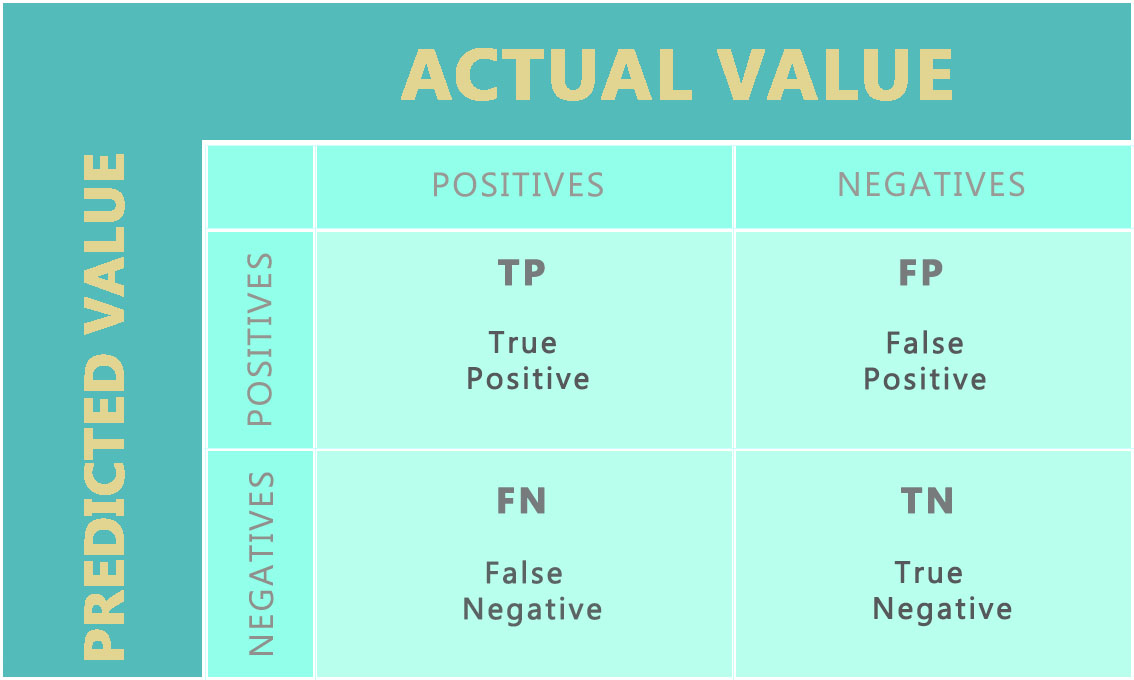
\includegraphics[scale=0.33]{Graphics/confusion-matrix.png}
    \caption{Confusion Matrix}
    \label{fig:confusion-matrix}
\end{figure}


Based on the above given categories, measurement metrics can be calculated. Some of them are given bellow:

\[ \textrm{False Positive Rate (FP-Rate)} = \frac{FP}{N}, \textrm{where } N \textrm{ stands for negatives.}  \]
\[ \textrm{True Positive Rate (TP-Rate)} = \frac{TP}{P}, \textrm{where } P \textrm{ stands for positives.}  \]


An discrete classifier have by definition a class label as output to a particular example (e.g \(Y\)/\(N\) for binary classification) \cite{Fawcett:2006:IRA:1159473.1159475}. The results can be easily represented on a basic ROC Graph (see figure\footnote{Figure is taken from the work of \cite{Fawcett:2006:IRA:1159473.1159475}}: \ref{fig:roc-graph}), where the \(x\) - axis is the FP-Rate and \(y\) is representing the TP-Rate. The best classifier/point on the graph is the one with the highest true positive and the lowest false negative rate (point \(D\) on our graph).
\begin{figure}[h!]
    \centering
    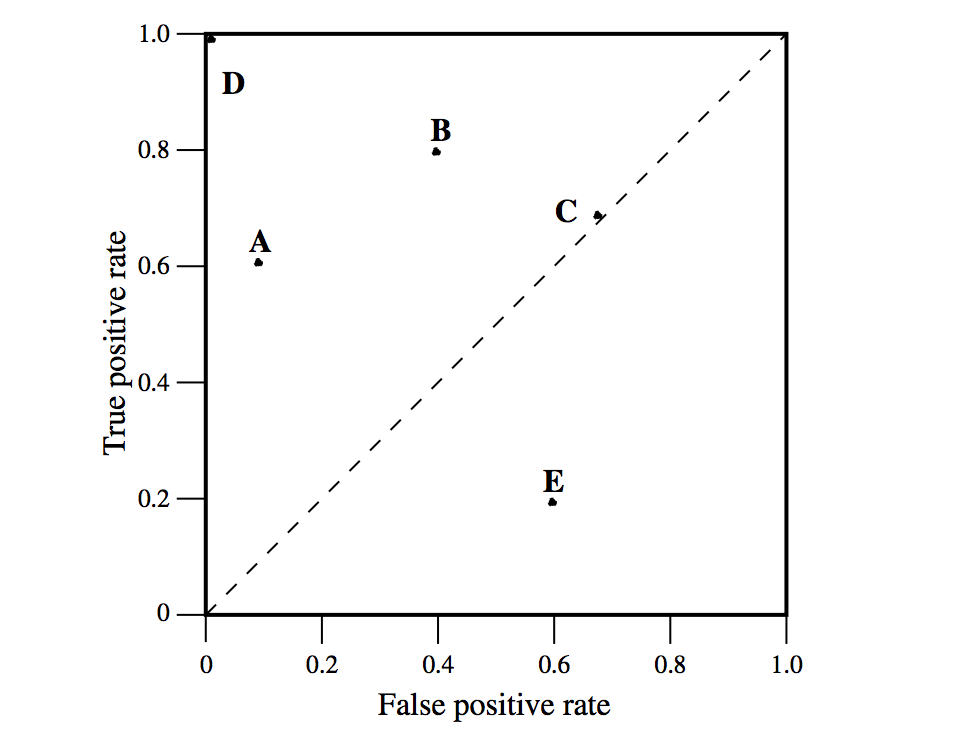
\includegraphics[scale=0.6]{Graphics/roc-graph.png}
    \caption{ROC-Graph for discrete classifier.}
    \label{fig:roc-graph}
\end{figure}

Moreover, a considerable case is the point \(C\) located on the diagonal dotted line. There the FP and TP rates are equivalent - ergo the classification probability is random.

Some classifier naturally yields a numeric value as a classification result of an example. These values are either strict probabilities or they can be uncalibrated scores, where a higher score indicate a higher probability. Although these values can be converted into binary labels by using a threshold e.g if the value is above the threshold then the label is \(Y\) else \(N\). So, each threshold would produce a different point into the ROC-Space, connecting the points together produce the ROC-Curve (see figure\footnote{Figure is taken from the work of \cite{Fawcett:2006:IRA:1159473.1159475}}:\ref{fig:roc-curve}). 

\begin{figure}[h!]
    \centering
    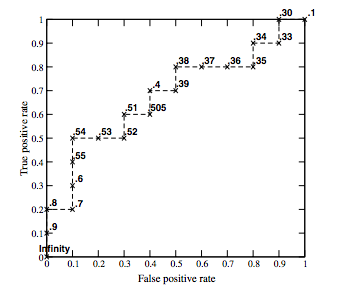
\includegraphics[scale=0.7]{Graphics/roc-curve.png}
    \caption{ROC-Curve for probabilistic classifier.}
    \label{fig:roc-curve}
\end{figure}

Another important property of ROC-Curve it is slightly sensitive to the distribution of particular classes in the data (e.g the proportions of FP-Rate <-> TP-Rate). This may an attractive feature if true negative is not much valuable to the problem, or negative examples are abundant but in the case of a fraud detection problem, where negative (fraud) examples are by definition rare, the ROC-Graph will not provide enough insides to measure classification right caused by skewed class distribution. Thus, additional metrics required.
Bellow, precision, and recall are given, both of them are sensitive to the class distribution due to the fact that the calculation is also related to the opposite classification category (TP-Rate is related to True Positives and the amount of positives where precision also include false negatives in the calculation):

\[ \textrm{Positive precision  (precision)} = \frac{TP}{TP+FN}  \]
\[ \textrm{Negative recall (recall)} = \frac{TN}{TN+FP}  \]

An example in figure\footnote{Figure is taken from the work of \cite{Fawcett:2006:IRA:1159473.1159475}} \ref{fig:roc-pr-curve} illustrate classification on two data sets differ by the amount of negatives. The curves on (a) and (c) (ROC-Curve) show up only a minimal change although a number of negatives is differed by 10 times, where the positive-recall graph on (b) and (d) differ substantially. 

\begin{figure}[h!]
    \centering
    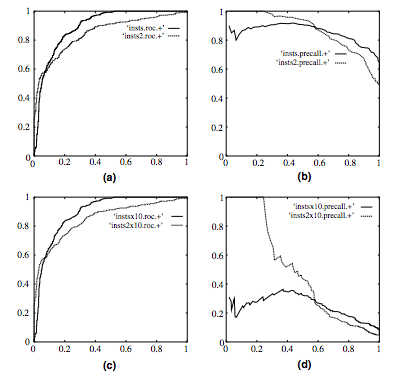
\includegraphics[scale=0.8]{Graphics/curves-vs-pr-analysis.png}
    \caption{ROC-Curve for probabilistic classifier.}
    \label{fig:roc-pr-curve}
\end{figure}

ROC analysis is a useful tool for measuring classifiers performance. With the concept of ROC graphs, a visualization technique is given to provide a richer
measure of classification performance than scalar measures
such as accuracy, error rate or error cost \cite{Fawcett:2006:IRA:1159473.1159475}. Moreover, precision - recall curves look promising to satisfy the needs of this thesis by the ability to evaluate classification algorithms used on a class-imbalanced data set.


\chapter{Experimental Protocol}\label{Chapter:5}


\section{Experiment Setting (plan)}

Dont forget to write here a chart down how many features left after each procedure of data processing.

\section{Experimental Results}





% FAZIIIIIIT!!!!!






\chapter{Evaluation of Results: Value for Business}


\chapter{Conclusion}\label{Chapter:7}

Anomalies about persons who get the loan and immediately  pay it back could not be found or it was not enough time to care about it 

Active Learning (ref to the Outlier Detection Book)

Parameter Tuning optimization, automatically optimization like hill climbing.









%\lipsum

%See also \cite{sample_bib}.
%%%%

%% appendix if used
%%\appendix
%%\typeout{===== File: appendix}
%%\include{appendix}

% bibliography and other stuff
\backmatter

\typeout{===== Section: literature}
%% read the documentation for customizing the style
\bibliographystyle{dinat}
\bibliography{sample}

\typeout{===== Section: nomenclature}
%% uncomment if a TOC entry is needed
%%\addcontentsline{toc}{chapter}{Glossar}
\renewcommand{\nomname}{Glossar}
\clearpage
\markboth{\nomname}{\nomname} %% see nomencl doc, page 9, section 4.1
\printnomenclature

%% index
\typeout{===== Section: index}
\printindex

\HAWasurency

\end{document}
